\section{Class diagram}
\subsection{Description}
\begin{flushleft}
Dans cette section, nous découvrirons les différentes classes liées à l'implémentation des différentes fonctionnalités.
\end{flushleft}

\begin{flushleft}
Tout d'abord, le schéma ci-dessous ne reprend que la classe de l'extension (étant donné que le schéma est suffisamment grand et est déjà disponible plus haut). La classe \textbf{Facture} est reliée à la classe \textbf{ClientApi} puisque que cette extension n'est disponible que pour les clients.
\end{flushleft}

\subsection{Les variables}
\begin{flushleft}
Dans la classe \textbf{Facture}, plusieurs arguments sont répertoriés.
\end{flushleft}

\begin{enumerate}[-]

\item La variable \emph{paiement-status} permet de voir le statut de paiement de la facture via un boolean (payed=true).

\item La variable \emph{ideal-accompt} affiche l'acompte calculé automatiquement par l'application via un double.

\item La variable \emph{paiement-method} affiche la méthode de paiement via un boolean (manual=true).

\item La variable \emph{paiement-informations} affiche, sous forme d'une ArrayList, les informations de paiement.

\item La variable \emph{factures-history}, de la même manière que la variable précédente, affiche un historique des factures du client.

\item La variable \emph{proposal} contient, sous forme d'un double, la proposition du client lorsqu'il modifie la proposition faite par l'application.

\end{enumerate}

\newpage
\subsection{Les méthodes}
\begin{flushleft}
Plusieurs méthodes de cette classe permettent l'implémentation des factures.
\end{flushleft}

\begin{enumerate}[-]

\item La méthode \emph{checkStatus} permet de vérifier le statut de paiement d'une facture.

\item La méthode \emph{calculateAmount} est la méthode par laquelle l'application va calculer le montant idéal.

\item La méthode \emph{checkProposal} permet à l'application de vérifier les conditions de la proposition du client.

\item La méthode \emph{changePaiementMethod} permet au client de modifier son mode de paiement.

\item La méthode \emph{changePaiementInformations} modifie les informations bancaires du client à sa volonté.

\item Dans le cas où le paiement manuel est choisi, la méthode \emph{generateQRCode} est appelée afin de générer un QR Code correspondant au paiement.

\item La méthode \emph{sendNotification} envoie une notification (via une application externe) lorsque qu'une facture est disponible.

\item La méthode \emph{seeHistory} permet au client de voir la liste de ses factures. Chaque facture sera ajoutée dans la liste des factures.

\item La méthode \emph{checkIsPayed} est une méthode liée au paiement de vérifier si le paiement est validé ou pas.

\item La class est munie d'un constructeur \emph{Facture} créant l'objet Facture pouvant être ajouté dans l'ArrayList.

\end{enumerate}

\newpage
\begin{figure}[h]
\subsection{Schéma}
\centering
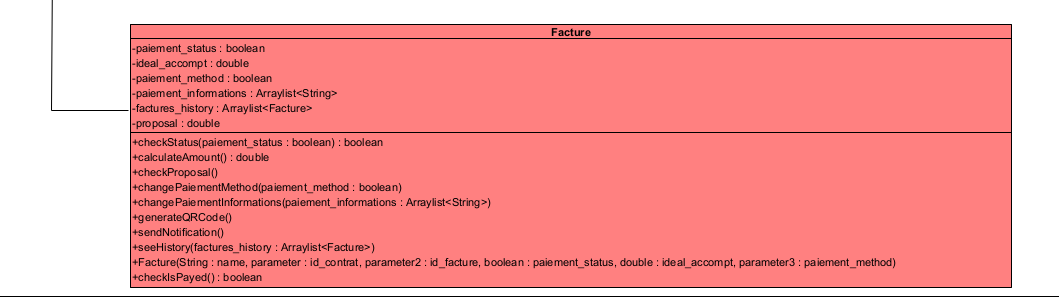
\includegraphics[width = 1.3\textwidth]{extension-maxime/class/img/class-extension.png}
\end{figure}


